\scalebox{0.85}{
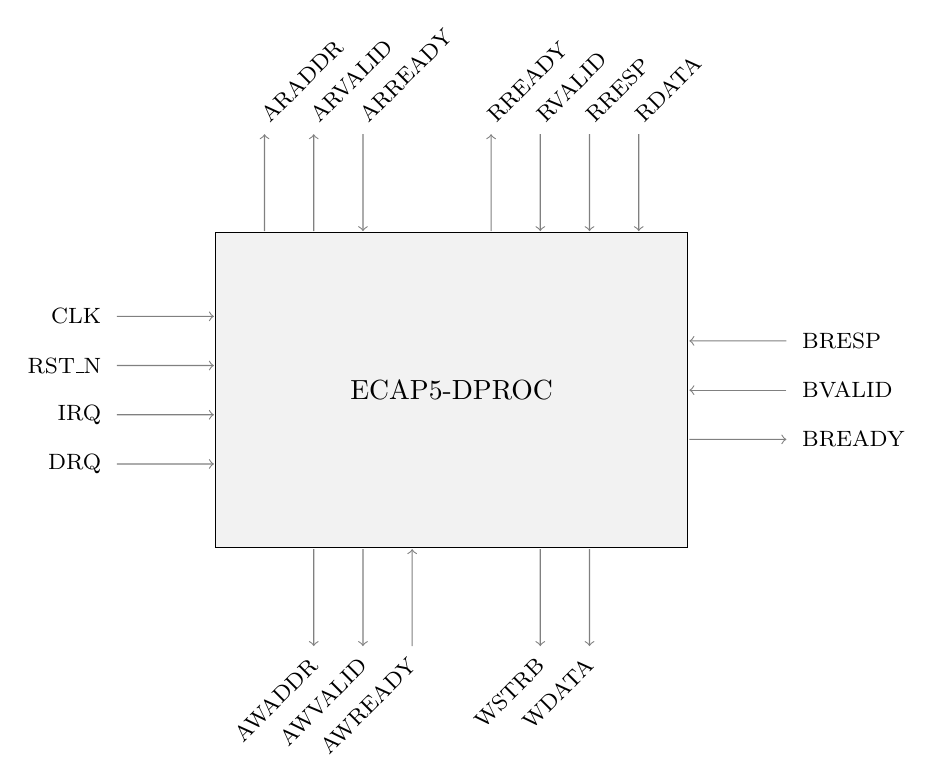
\begin{tikzpicture}[scale=1.25, draw=gray, inner sep=0, outer sep=0]
  \node[rectangle, draw=black,
    minimum height = 4cm,
    minimum width = 6cm,
    fill = gray!10] (box) at (0, 0) {ECAP5-DPROC};

  % left
  \node (lport1) at ([yshift=0.75cm]box.west) {};
  \node (lport2) at ([yshift=0.25cm]box.west) {};
  \node (lport3) at ([yshift=-0.25cm]box.west) {};
  \node (lport4) at ([yshift=-0.75cm]box.west) {};

  \draw[->] ([xshift=-1cm]lport1.center) node[left=0.2cm, anchor=east]{\footnotesize CLK} -- (lport1);
  \draw[->] ([xshift=-1cm]lport2.center) node[left=0.2cm, anchor=east]{\footnotesize RST\_N} -- (lport2);
  \draw[->] ([xshift=-1cm]lport3.center) node[left=0.2cm, anchor=east]{\footnotesize IRQ} -- (lport3);
  \draw[->] ([xshift=-1cm]lport4.center) node[left=0.2cm, anchor=east]{\footnotesize DRQ} -- (lport4);

  % top
  \node (uport1) at ([xshift=0.5cm]box.north west) {};
  \node (uport2) at ([xshift=1cm]box.north west) {};
  \node (uport3) at ([xshift=1.5cm]box.north west) {};
  \node (uport4) at ([xshift=-0.5cm]box.north east) {};
  \node (uport5) at ([xshift=-1cm]box.north east) {};
  \node (uport6) at ([xshift=-1.5cm]box.north east) {};
  \node (uport7) at ([xshift=-2cm]box.north east) {};
  
  \draw[<-] ([yshift=1cm]uport1.center) node[above=0.2cm, anchor=west, rotate=45]{\footnotesize ARADDR} -- (uport1);
  \draw[<-] ([yshift=1cm]uport2.center) node[above=0.2cm, anchor=west, rotate=45]{\footnotesize ARVALID} -- (uport2);
  \draw[->] ([yshift=1cm]uport3.center) node[above=0.2cm, anchor=west, rotate=45]{\footnotesize ARREADY} -- (uport3);
  \draw[->] ([yshift=1cm]uport4.center) node[above=0.2cm, anchor=west, rotate=45]{\footnotesize RDATA} -- (uport4);
  \draw[->] ([yshift=1cm]uport5.center) node[above=0.2cm, anchor=west, rotate=45]{\footnotesize RRESP} -- (uport5);
  \draw[->] ([yshift=1cm]uport6.center) node[above=0.2cm, anchor=west, rotate=45]{\footnotesize RVALID} -- (uport6);
  \draw[<-] ([yshift=1cm]uport7.center) node[above=0.2cm, anchor=west, rotate=45]{\footnotesize RREADY} -- (uport7);

  % bottom
  \node (bport1) at ([xshift=1cm]box.south west) {};
  \node (bport2) at ([xshift=1.5cm]box.south west) {};
  \node (bport3) at ([xshift=2cm]box.south west) {};
  \node (bport4) at ([xshift=-1cm]box.south east) {};
  \node (bport5) at ([xshift=-1.5cm]box.south east) {};

  \draw[<-] ([yshift=-1cm]bport1.center) node[below=0.2cm, anchor=east, rotate=45]{\footnotesize AWADDR} -- (bport1);
  \draw[<-] ([yshift=-1cm]bport2.center) node[below=0.2cm, anchor=east, rotate=45]{\footnotesize AWVALID} -- (bport2);
  \draw[->] ([yshift=-1cm]bport3.center) node[below=0.2cm, anchor=east, rotate=45]{\footnotesize AWREADY} -- (bport3);
  \draw[<-] ([yshift=-1cm]bport4.center) node[below=0.2cm, anchor=east, rotate=45]{\footnotesize WDATA} -- (bport4);
  \draw[<-] ([yshift=-1cm]bport5.center) node[below=0.2cm, anchor=east, rotate=45]{\footnotesize WSTRB} -- (bport5);

  % right
  \node (rport1) at ([yshift=0.5cm]box.east) {};
  \node (rport2) at (box.east) {};
  \node (rport3) at ([yshift=-0.5cm]box.east) {};

  \draw[->] ([xshift=1cm]rport1.center) node[right=0.2cm, anchor=west]{\footnotesize BRESP} -- (rport1);
  \draw[->] ([xshift=1cm]rport2.center) node[right=0.2cm, anchor=west]{\footnotesize BVALID} -- (rport2);
  \draw[<-] ([xshift=1cm]rport3.center) node[right=0.2cm, anchor=west]{\footnotesize BREADY} -- (rport3);
\end{tikzpicture}
}
